\section{Methodology} \label{sec:methodology}
\subsection{Outcome Assessment}
talk about outcome assessment here. Show all of the math, talk about the equations in some detail. Refer to Sec. 5.2 for formulation, and 5.3 for evaluation \cite{Aitken2016-cv}
\subsubsection{UPM/LPM}

\begin{align}
    U(f) &:= \int_{-\infty}^0 v(r)\deriv{}{r}(w(F(r)))dr \\ \nonumber
    &\quad + \int_{0}^{+\infty}v(r)\deriv{}{r}(-w(1-F(r)))dr
\end{align}

\begin{align}
    UPM/LPM &= \frac{\int_{0}^{+\infty}\tilde{z}\tilde{f}(\tilde{z})d\tilde{z}}{\int_{-\infty}^{0} \tilde{z}\tilde{f}(\tilde{z})d\tilde{z}} \label{eq:upm/lpm} \\
    \xO{} &= 2/(1+e^{(-k(log(UPM/LPM)))}) - 1 \label{eq:xp}
\end{align}

\subsubsection{Properties}
\brett{Refer to paper for in-depth properties and behaviors, here probably just put a table with some words about +1/-1 stuff}

\subsection{Solver Quality}
\brett{\xQ{} is a bit more complicated than \xO{} to explain, and in derivation, need to spend a little more time, but also defer to \cite{Israelsen2018-qz} for more detail.}
How, then, can \xQ{} be calculated? Following from discussion in the previous section, a surrogate model \surrogate{} can be learned to predict the reward distribution \rwdstarapprox{} of the trusted reference solver \solvestar{} on task \task{}.

The candidate solver \solve{} must then be evaluated w.r.t. the trusted solver \solvestar{}. This is done by comparing \rwdstarapprox{} (the predicted performance of \solvestar{} on task \task) and \rwd{} (the simulated performance of solver \solve{} on task \task).

Figure \ref{fig:sq_v2} illustrates some of the key quantities involved in calculating \xQ. The basic premise is: \emph{find the difference between the trusted ($T$) and candidate ($C$) solvers while taking into account the overall range of rewards of the trusted solver over many tasks}.

\subsubsection{Calculating \texorpdfstring{\xQ}{xQ}}
   \begin{figure}[tb]
        \centering
        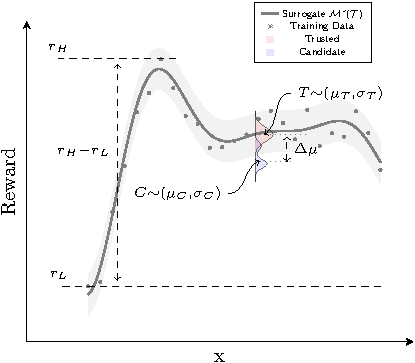
\includegraphics[width=0.9\linewidth]{Figures/sq_v2_fig-crop}
        \caption{Key values involved in calculating \xQ, where $x$ represents a `parameter of interest' for task \task, or solver \solve.}
        \label{fig:sq_v2}
        \vspace{-0.2cm}
    \end{figure}
The main aim of \xQ{} is to indicate how a solver \solve{} will perform on a given (possibly un-encountered) task \task{} of a given class \taskclass{} (i.e. all road networks with a UGV, Pursuer, and exit, et cetera as described previously). The need for \xQ{} is not necessarily easy to understand; an analogy helps to clarify:

\emph{Clarifying Example:} One could informally think of \xQ{} as an indication of the \emph{ability} of an athlete. This is opposed to the athlete's assessment of the desirability of the outcome of a game (\xO). While an athlete may be very capable (high \xQ), the score of the game may be such that the athlete knows that it is nearly impossible to catch up and win the game (low \xO). Conversely, an athlete may not be very capable (low \xQ), and due to being na\"{i}ve has an incorrect assessment of the desirability of the outcome (\xO{} cannot be trusted).

In order to compare two solvers the resultant reward distributions that each of those solvers produce are compared. If two solvers produce an identical reward distribution \emph{for a given task}, then they can be considered equal in their `quality', or considered equally `capable'. Conversely, if the two distributions are very different \emph{for the same task}, then their quality, or capability, is also different. \brett{again\ldots refer to \cite{Israelsen2018-qz} for more detail}.

\paragraph{Hellinger Metric \texorpdfstring{$\bm{\hell}$}{H^2}} \label{sec:hellinger}
The \emph{Hellinger Metric}, \hell{},  is a measure of the distance between two distributions. It is bounded between 0 and 1, where 0 means the distributions are identical. The maximum distance, 1, is achieved when one distribution $P$ assigns zero probability at every point in which another distribution $Q$ assigns probability. \hell{} has different forms based on the type of analytical distributions being compared. For the purposes of calculating \xQ{} from two distributions $P \sim (\mu_1,\sigma_1)$ and $Q\sim(\mu_2,\sigma_2)$ the following form is useful:
\begin{align}
    \hellmet = 1-\sqrt{\frac{2\sigma_P\sigma_Q}{\sigma_P^2+\sigma_Q^2}}\exp{\left(-\frac{1}{4}\frac{(\mu_P-\mu_Q)^2}{\sigma_P^2+\sigma_Q^2}\right)}
\end{align}

Using \hell{} the overlap between $T$ and $C$ can be calculated. The sing of the difference is accounted for by \dmu.

\begin{align}
    \text{q} &= \text{sgn}(\Delta \mu)f^{\alpha}\sqrt{H^{2}(T,C)} \label{eq:q} \\
    x_{Q} &= \frac{2}{1+exp(-\text{q}/5)}\label{eq:SQ}
\end{align}

Where $\Delta \mu = \mu_c-\mu_t$, and $f = \Delta \mu/(r_H-r_L)$. The exponent $\alpha$ is a parameter that affects the influence that $f$ has with respect to \hell. In essence, should the relationship of the effects of $f$ and \hell{} be $1:1$? In practice $\alpha=1$ does not yield desirable results. \hell{} should be more influential on $\text{q}$ as $f$ grows smaller, and $f$ should be more influential as it increases. We have found $\alpha=1/2$ gives results that `make sense'; future work could investigate the `best' value for $\alpha$ via user studies.

\paragraph{Properties}
While \hell{} is on the domain $[0,1]$, the quantity $f$ is $[0,\infty]$. Because of this it is desirable to use a `squashing function' to keep the reported \xQ{} value within some bounded range and avoid arbitrarily large values that can be confusing to humans. The general logistic equation is useful for this.
The numerator is 2 so that when $q=0$ (distributions are identical) \xQ{} will be 1. Dividing the quantity $q$ by 5 so makes it so that \xQ{} `saturates' at around $\text{q}=\pm1$.

\brett{Reference the ArXiv paper for numerical experiments}
Several numerical experiments were performed to verify that the Solver Quality metric (\xQ{}) performed as expected in several different situations.
